\section{Experiments}

\subsection{Exploratory Research Phase}
After about a month of researching for existing solutions, applying for NVIDIA CloudXR \parencite{cloudxr} and testing the difficulty of different prototype architectures it became clear that making a prototype from scratch is not a feasible task for the duration and team size of the project. This conclusion is based on two major observations:

\paragraph{NVIDIA CloudXR SDK is the only working solution}
During the research a couple of existing products were found, that demonstrated the feasibility of key areas of interest for this project: Low Latency and High Security \parencite{gtc2020esi}. All of the products found were launched shortly before the start or during the graduation, so it is safe to say that the technology and market is currently emerging. Another overlap of these products was that they all used NVIDIA's CloudXR SDK to enable them to stream \acrshort{vr} content. In the conference talks, where these products were presented, CloudXR was always mentioned as the last piece of the puzzle to enable the creation of ambitions cloud \acrshort{vr} projects.

\paragraph{Creating a custom Prototype is impossible}
When experimenting with the \hyperref[fig:pr11]{first} and \hyperref[fig:pr12]{second} prototype design, both in Unreal Engine 4 and Unity 3D, it was possible to quickly create a WebRTC connection from a 'server' machine to a 'client' machine in the same network. However before I ever got to implementing the whole application loop it was already evident that the performance would be a critical factor. As explored in the \nameref{sec:theo} the \acrfull{mtp} latency for a single frame is not allowed exceed 20\acrshort{ms}, where as the base latency of the connection in the prototypes would be atleast around 100-200\acrshort{ms}. This measurement was taken in a local network instead of a connection to a cloud server and without streaming the significantly bigger \acrshort{vr} resolution of 2160x1200, all of which things that would have impacted the latency negatively even more. Considering this it would be impossible to create and optimize a prototype to undercut the \acrshort{mtp} barrier within the remaining time frame of the project. Additionally there was a serious lack of documentation and examples for SteamVR/OpenVR, the most critical component in the proposed designs. Lastly it also became clear that alternative solutions, like ReactVR \parencite{reactVR} and A-Frame \parencite{aframe}, are not suitable for the use-cases of the stakeholders as they do not allow for the complexity needed as presented in the \nameref{sec:int}. \\

\subsection{Building the prototype}
At the end of the exploratory research phase I finally got into contact with an NVIDIA employee who was able to grant me access to the CloudXR SDK. I was able to successfully set up the \hyperref[fig:pr0]{pipeline} in the local network of the XR lab within a couple of days. Some initial user testing from myself and volunteering teachers revealed that the solution was potent, as most testers experienced no or only minor degradations in their user experience

I then worked together with Thales and Microsoft Azure to gain access to a \acrfull{vm} with the necessary hardware inside of Azure. After two days, due to a driver and licensing issue, I was able to set up the prototype on the aforementioned \acrshort{vm}. However the user experience was horrible, due to poor latency and \acrshort{fps}. The root of this issue was a mismatch of (v)\acrshort{gpu} driver versions and \acrfull{os}'s. After installing compatible versions of v\acrshort{gpu} drivers and CloudXR, as well as an virtual audio driver, the prototype finally worked as intended.

\begin{table}[h]	
\begin{center}
\caption{Server and Client Specifications}
\begin{tabular}{ |c|c|c|c| } 
\hline
\multicolumn{2}{|c|}{Server Specifications} & \multicolumn{2}{|c|}{Client Specifications}\\ 
\hline\hline
\textbf{\acrshort{os}} & Windows Server 2019  &  \textbf{\acrshort{os}} & Windows 10 Pro\\ 
\hline
\textbf{\acrshort{gpu}} & P100 & \textbf{\acrshort{gpu}} & GeForce RTX 2080 Ti\\ 
\hline
\textbf{Driver} & 451.48 &  \textbf{Driver} & 432.00\\ 
\hline
\textbf{\acrshort{cpu}} & Intel Xeon E5-2690 v9 & \textbf{\acrshort{cpu}} & Intel I7-7820X\\
\hline
\textbf{Memory} & 112 GiB & \textbf{Memory} & 64 GiB\\
\hline
\textbf{Location} & Europe West & \textbf{\acrshort{hmd}} & Vive Pro\\
\hline
\textbf{Azure VM Series} & NC6s v2 & & \\
\hline
\end{tabular}
\end{center}

\end{table}

\subsection{Testing the prototype}
Before starting to build the prototype, I had a meeting with Thales to discuss how to test it once it is running. Together we agreed on conducting 2 types of test with 2 different tools to measure the performance of the prototype.

\subsubsection{Test 1: End-to-End Latency}
\begin{figure}[h!]
\caption{End-to-End Latency Visualized \parencite{e2e}}
\label{fig:e2e}
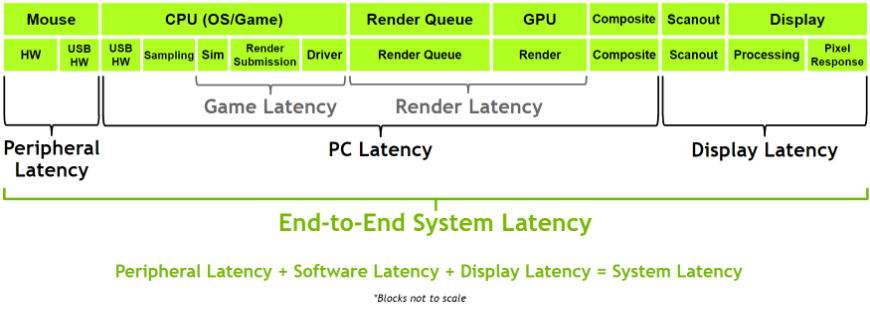
\includegraphics[scale=0.6]{E2E}
\end{figure}
The first test will be to measure the overall End-to-End latency of the system. This will be achieved with a tool from NVIDIA, that is built to measure \acrshort{mtp} latency, by waiting to detect changes in luminance after user input (mouse click). Due to an NDA I cannot reveal any specific details about the device, but the embargo is expected to be lifted before the end of the project.

It is also expected that the results of this measurement are quite high. This is due to the fact that this test's measurements include the hardware and software latency of two computers, as well as the network latency between those.

\subsubsection{Test 2: Network Latency}
The second test will measure the network latency, by testing the round trip delay. This will be done with the open-source tool Wireshark \parencite{wireshark}. By comparing the resulting measurements with the first test, the impact of network latency on the whole system will be revealed.